Gaussian beam and low-loss mode conditions.

\begin{parts}
	\part
	\begin{figure}[H]
		\centering
		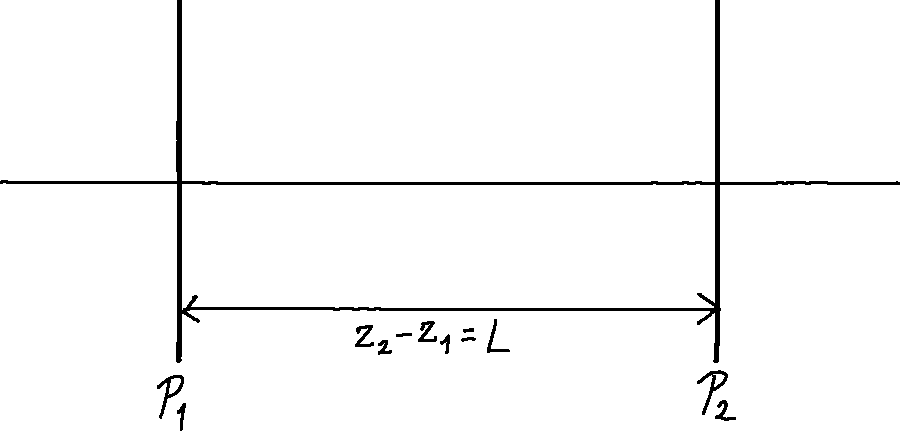
\includegraphics[width=.7\linewidth]{q2-setup}
	\end{figure}
	Replacing the mirror with a lens gives:
	\begin{align*}
		\begin{pmatrix}
			q^\prime \\ 0
		\end{pmatrix} &= \mathcal{UF}
		\begin{pmatrix}
			1 & L \\
			0 & 1
		\end{pmatrix}
		\begin{pmatrix}
			1 & L \\[1em]
			-\dfrac{1}{f} & 1
		\end{pmatrix}
		\begin{pmatrix}
			1 & L \\
			0 & 1
		\end{pmatrix}
		\begin{pmatrix}
			q \\ 1
		\end{pmatrix} \\
		&= \mathcal{UF} \begin{pmatrix}
			1 & L \\
			0 & 1
		\end{pmatrix}
		\begin{pmatrix}
			1 & L \\[1em]
			-\frac{1}{f} & 1-\dfrac{L}{f}
		\end{pmatrix}
		\begin{pmatrix}
			q \\ 1
		\end{pmatrix} \\
		&=\mathcal{UF} \begin{pmatrix}
			1-\dfrac{L}{f} & L+L-\dfrac{L^2}{f} \\[1em]
			-\dfrac{1}{f} & 1-\dfrac{L}{f}
		\end{pmatrix}
		\begin{pmatrix}
			q \\ 1
		\end{pmatrix} \\
		\Rightarrow q^\prime &= \frac{(1-L/f)q + 2L - L^2/f}{-q/f + 1 - L/f} \\
		&= \frac{(1-L/f)iz_R + (2L - L^2/f)}{(1-L/f) - iz_R/f} \\
		&= \frac{\sbracket{(2L - L^2/f) + iz_R(1 - L/f)} \sbracket{(1 - L/f) + iz_R/f}}{(1-L/f)^2 + (z_R/f)^2} \\
		&= \frac{(2L-L^2/f)(1-L/f) - z_R^2(1-L/f)/f + i\sbracket{z_R(1-L/f)^2 + z_R/f (2L-L^2/f)}}{(1-L/f)^2 + (z_R/f)^2}
	\end{align*}
	
	Note that the real part vanishes for $R = 2L = 2f$, hence the reflected beam has the waist on $\mathcal{P}$ (by reflecting $\mathcal{P}^\prime$ to $\mathcal{P}$).
	
	Now the imaginary part should be:
	\begin{align*}
		z_R^\prime &= \frac{z_R/L (2L-L)}{0 + (z_R/L)^2} \\
		&= z_R \cdot \frac{L^2}{z_R^2} \\
		&= \frac{L^2}{z_R}
	\end{align*}
	
	For $R \neq 2L$, we demand $q^\prime = q \Rightarrow z_R^\prime = z_R$ since the waist position is unchanged:
	\begin{align*}
		z_R &= \frac{(1-L/f)^2 z_R + z_R/f (2L-L^2/f)}{(1-L/f)^2 + (z_R/f)^2} \\
		&= \rbracket{1-\frac{L}{f}}^2 + \rbracket{\frac{z_R}{f}}^2 = \rbracket{1-\frac{L}{f}}^2 + \frac{2L-L^2/f}{f} \\
		\Rightarrow z_R^2 &= f^2 \frac{2L-L^2/f}{f} \\
		&= Lf \rbracket{2 - \frac{L}{f}} \\
		&= LR \rbracket{1 - \frac{L}{R}} \\
		\Rightarrow z_R &= \sqrt{LR\rbracket{1-\frac{L}{R}}}
	\end{align*}
	
	\part
	\begin{figure}[H]
		\centering
		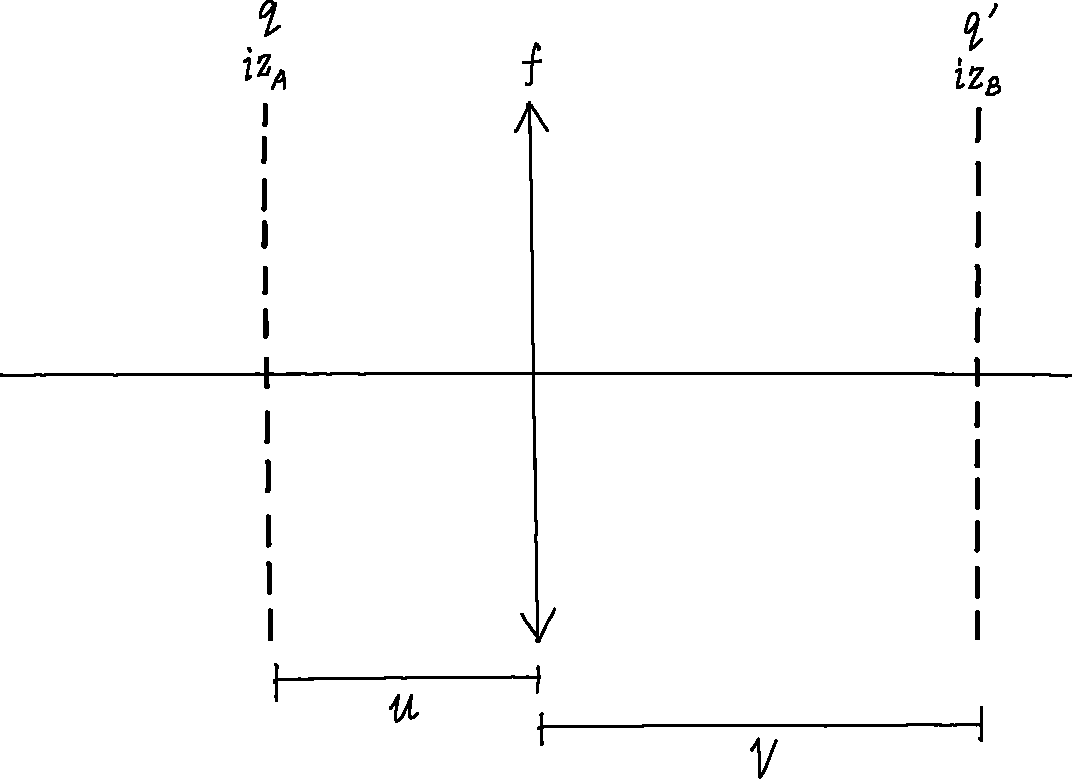
\includegraphics[width=.7\linewidth]{q2-uv}
	\end{figure}
	Similarly we have:
	\begin{align*}
		\begin{pmatrix}
			q^\prime \\ 1
		\end{pmatrix} &= \mathcal{UF}
		\begin{pmatrix}
			1 & v \\
			0 & 1
		\end{pmatrix}
		\begin{pmatrix}
			1 & 0 \\[1em]
			-\dfrac{1}{f} & 1
		\end{pmatrix}
		\begin{pmatrix}
			1 & u \\
			0 & 1
		\end{pmatrix}
		\begin{pmatrix}
			q \\ 1
		\end{pmatrix} \\
		\Rightarrow \begin{pmatrix}
			q^\prime \\ 1
		\end{pmatrix} &= \mathcal{UF}
		\begin{pmatrix}
			1-\dfrac{v}{f} & v \\[1em]
			-\dfrac{1}{f} & 1
		\end{pmatrix}
		\begin{pmatrix}
			q+u \\ 1
		\end{pmatrix} \\
		q^\prime &= \frac{q + u - (q+u)/f v + v}{-(q+u)/f + 1} \\
		&= \frac{f(u+v) - uv + iz_A(f-v)}{f-u-iz_A} = iz_B \\
		\Rightarrow i(f-u)z_B + z_A z_B &= fu + fv - uv + iz_A (f-v)
	\end{align*}
	
	Equating real part gives:
	\begin{align}
		z_A z_B &= uf + v(f-u) \notag \\
		\Rightarrow v(u-f) + z_A z_B &= uf
		\label{eqn:q2-part-b-i}
	\end{align}
	
	Equating imaginary part gives:
	\begin{align}
		(f-u)z_B &= z_A (f-v) \notag \\
		\Rightarrow vz_A - z_B (u-f) &= z_A f
		\label{eqn:q2-part-b-ii}
	\end{align}
	
	From \eqref{eqn:q2-part-b-ii}:
	\begin{align*}
		z_A v &= z_A f + z_B \delta \mtext{where $\delta = f-u$} \\
		\xRightarrow{\eqref{eqn:q2-part-b-i}} -\frac{\delta}{z_A} \rbracket{z_A f + z_B \delta} + z_A z_B &= \rbracket{f - \delta}f \\
		-f\delta - \frac{z_B}{z_A}\delta^2 + z_A z_B &= f^2 - \delta f \\
		\delta &= \sqrt{\frac{z_A}{z_B} \rbracket{f^2 - z_A z_B}}
	\end{align*}
	
	We want $\delta$ to be real, so $f^2 > z_A z_B$.
	
	\part Rayleigh range of the 1st cavity: $z_1 = \sqrt{L_1 R_1 (1 - L_1/R_1)} = \SI{1000}{\milli\metre}$.
	
	Rayleigh range of the 2nd cavity: $z_2 = \sqrt{L_2 R_2 (1 - L_2/R_2)} = \SI{866}{\milli\metre}$.
	
	From b, we have:
	\begin{align*}
		\delta &= \sqrt{\frac{z_1}{z_2} \rbracket{f^2 - z_1 z_2}} = u-f = \SI{126.4}{\milli\metre} \\
		\Rightarrow u &= \SI{1.626}{\metre}
	\end{align*}
	
	Also $v = f + z_2/z_1 \delta = \SI{12.45}{\metre}$.
	
	\part Compared to a symmetrical confocal cavity, this system may help us to focus the Gaussian beam down or defocusing it, thereby enabling us to control the laser beam size.
\end{parts}